
\section{Baseline Results}

\subsection{Baseline: The 1-to-1 benchmark}

We start by establishing a baseline for each tested system and vendor which we can later use as a comparison for different environment configurations. We collect data in 20 minute runs (corresponding to just above 1000 samples per run), while retaining the default setting of one synchronization and one measurement of the path delay per second, as our results suggest that a higher frequency does not significantly improve clock synchronization while negatively impacting the stability of the measurement\todo{This is stated but not shown. Do we need to show?}.

\begin{figure}
    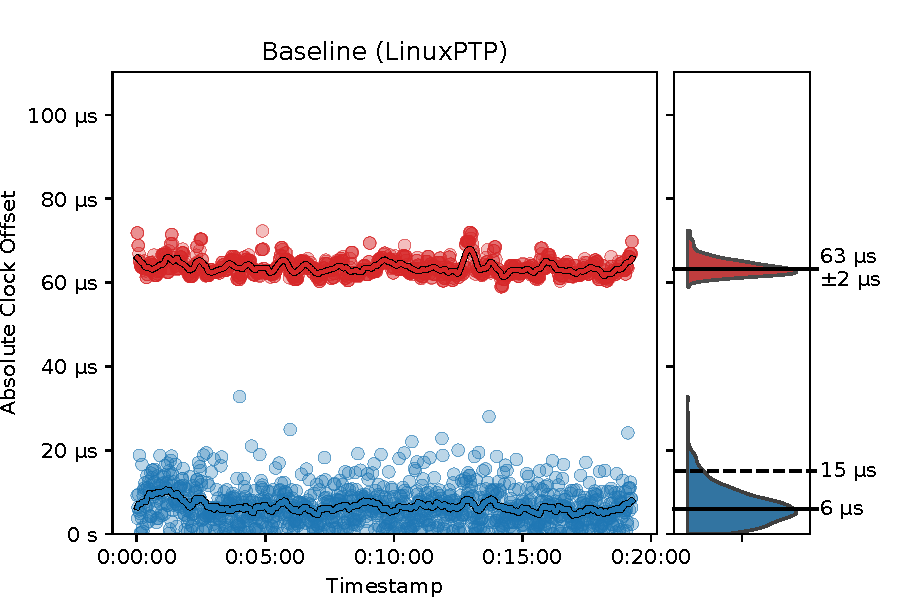
\includegraphics[width=\linewidth]{res/generated/baseline/sample.pdf}
    \caption{A sample run of LinuxPTP in its default configuration. Because PTP uses path delay compensation, the clock synchronization accuracy is much better than the one-way path delay.}
    \label{fig:baseline_sample}
\end{figure}

Figure \ref{fig:baseline_sample} shows a sample run of the baseline for the LinuxPTP vendor.

\subsection{Vendors}

\subsection{Systems}

\subsection{Reproducibility}

\pgfkeys{
    /reproducibility/rpi-4/.cd,
    ptpd/min/.initial={5.3},
    ptpd/median/.initial={6.1},
    ptpd/max/.initial={24},
    linuxptp/min/.initial={4.2},
    linuxptp/median/.initial={5.1},
    linuxptp/max/.initial={6.0},
}
\renewcommand{\ptpKeyPrefix}{/reproducibility/rpi-4}

\begin{figure}
    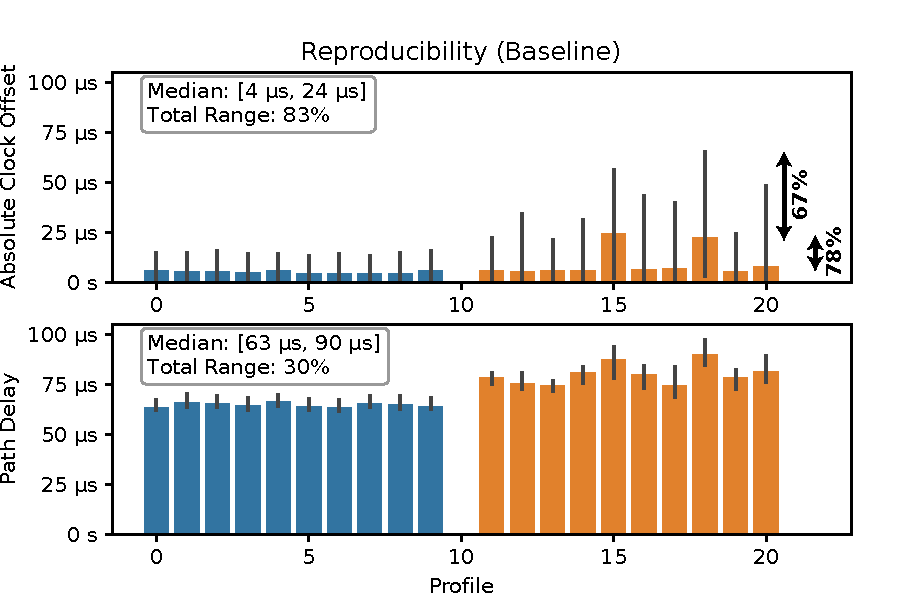
\includegraphics[width=\linewidth]{res/generated/baseline/key_metric_variance.pdf}
    \caption{Validating the baseline results by repeatedly measuring the baseline for both vendors on the Raspberry Pi 4 system. Top: The median absolute clock offset for each run, with error bars reaching from quantiles 0.05 to 0.95. Bottom: The same for the estimated path delay.}
    \label{fig:baseline_reproducibility}
\end{figure}

The first question to be answered is how reproducible the baseline is. To evaluate this, we repeat the measurement of the observations six times for each vendor (totaling in a four-hour runtime) and aggregate them. Between each measurement run, the entire cluster is restarted to ensure that no state that would harm the independence of observations is carried over. Otherwise, the setup is left untouched and all that happens is that the PTP installation is started and stopped.

Figure \ref{fig:baseline_reproducibility} shows the results. We observe that LinuxPTP produces significantly more stable results for both the clock offset estimation and the path delay, while PTPd shows more variance in median and 95-th quantile observed clock offset, while additionally being less sure about the path delay. A simple restart can suddenly cause the median latency to jump from the median \fTimeKey{ptpd/median} up to \fTimeKey{ptpd/max}, which corresponds to an increase of \fRatio{\ptpKey{ptpd/max}/\ptpKey{ptpd/median}} not only momentarily, but throughout an entire run. This already comes uncomfortably close to our safety factor of \safetyMargin, and we have not even started stressing the system yet. Fortunately, LinuxPTP produces a lot more stable results, with a smaller range of \fTimeKey{linuxptp/median} and \fTimeKey{linuxptp/max} between the median observed run and the worst observed run corresponding to just \fRelative{\ptpKey{linuxptp/max}/\ptpKey{linuxptp/median}}.

\begin{table}
\centering
\caption{Baseline Values by Vendor and System}
\begin{tabular}{rrrrr}
           & \multicolumn{2}{c}{Med. Clock Offset} & \multicolumn{2}{c}{$P_{95}$ Clock Offset}\\
    System & LinuxPTP & PTPd & LinuxPTP & PTPd\\
    Raspberry-Pi 4 & \fTimeKey{linuxptp/median} & \fTimeKey{ptpd/median} & \\
\end{tabular}

\end{table}